 \documentclass[11pt, oneside]{article}   	% use "amsart" instead of "article" for AMSLaTeX format
\usepackage{geometry}                		% See geometry.pdf to learn the layout options. There are lots.
\geometry{letterpaper}                   		% ... or a4paper or a5paper or ... 
%\geometry{landscape}                		% Activate for for rotated page geometry
%\usepackage[parfill]{parskip}    		% Activate to begin paragraphs with an empty line rather than an indent
\usepackage{graphicx}				% Use pdf, png, jpg, or eps§ with pdflatex; use eps in DVI mode
								% TeX will automatically convert eps --> pdf in pdflatex		
\usepackage{amssymb}
\usepackage{amsmath}

\title{Binomial Theorem by induction}
%\author{The Author}
\date{}							% Activate to display a given date or no date

\graphicspath{{/Users/telliott_admin/Dropbox/Tex/png/}}

\usepackage{listings,relsize} 
\lstloadlanguages{R} 
\lstset{language=R,basicstyle=\smaller[1],commentstyle=\rmfamily\smaller, 
  showstringspaces=false,% 
  xleftmargin=4ex,literate={<-}{{$\leftarrow$}}1 {~}{{$\sim$}}1} 
\lstset{escapeinside={(*}{*)}}   % for (*\ref{ }*) inside lstlistings (S code) 
\begin{document}

\maketitle
%\section{}
% \subsection*{R code}
% \begin{lstlisting}  \end{lstlisting}
% \begin{center} 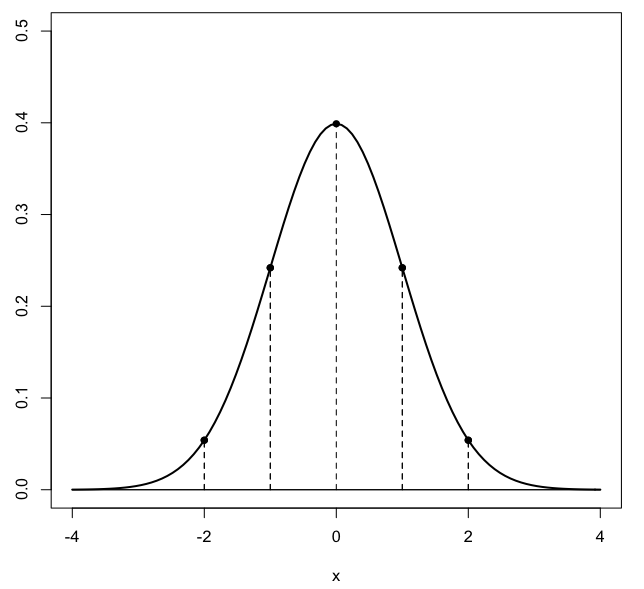
\includegraphics [scale=0.4] {gauss3.png} \end{center}
% \begin{bmatrix} a  &  b \\ c  &  d \end{bmatrix}
% \bigg |_

\large
\noindent

This proof has some issues.  Look at the pdf from the web to try to make it better.

The formula we would like to prove is
\[ (x+y)^n = \sum_{k=0}^{n} \ {n \choose k} \ x^{n-k}y^k \]
In the inductive step, we assume the formula is correct for 
\[ (x+y)^{n-1} = \sum_{k=0}^{n-1} \ {n-1 \choose k} \ x^{(n-1)-k}y^k \]
Then we multiply by $(x+y)$
\[ (x+y) \ \sum_{k=0}^{n-1} \ {n-1 \choose k} \ x^{(n-1)-k}y^k \]
and try to show that we can reduce to the formula we want to prove.  We obtain two terms from the sum
\[ L = x \ \sum_{k=0}^{n-1} \ {n-1 \choose k} \ x^{(n-1)-k}y^k = \sum_{k=0}^{n-1} \ {n-1 \choose k} \ x^{n-k}y^k \]
\[ R = y \ \sum_{k=0}^{n-1} \ {n-1 \choose k} \ x^{(n-1)-k}y^k = \sum_{k=0}^{n-1} \ {n-1 \choose k} \ x^{(n-1)-k}y^{k+1} \]
\subsection*{Massage the right term}
We want to manipulate $R$ a bit so substitute $j$ for $k$ as the index variable
\[ \sum_{j=0}^{n-1} \ {n-1 \choose j} \ x^{(n-1)-j}y^{j+1} \]
Rearrange things so we have $(j+1)$ in the crucial places
\[ \sum_{j=0}^{n-1} \ {n-1 \choose j} \ x^{n-(j+1)}y^{j+1} \]
\[ \sum_{j=0}^{n-1} \ {n-1 \choose (j+1)-1} \ x^{n-(j+1)}y^{j+1} \]
Now go back to $k$ where $k=j+1$
\[ \sum_{k=1}^{n} \ {n-1 \choose k-1} \ x^{n-k}y^{k} \]
If (like me) you have a hard time seeing why that works, let's expand a short series (say $n=3$).  In the first summation we go from $j=0 \to 2$
\[ \sum_{j=0}^{2} \ {n-1 \choose j} \ x^{n-(j+1)}y^{j+1} = {2 \choose 0}x^2y^1 + {2 \choose 1}x^1y^2 + {2 \choose 2}x^0y^3\]
In the second one we go from $k=1 \to 3$
\[ \sum_{k=1}^{3} \ {n-1 \choose k-1} \ x^{n-k}y^k = {2 \choose 0}x^2y^1 + {2 \choose 1}x^1y^2 + {2 \choose 2}x^0y^3\]
These two series are the same.
\subsection*{Adjusting the limits of the sum}
So now we have
\[ R = \sum_{k=1}^{n} \ {n-1 \choose k-1} \ x^{n-k}y^{k} \]
We want this sum to run from $0 \to n$ so we add and subtract the $k=0$ term
\[ R = \sum_{k=0}^{n} \ [ \ {n-1 \choose k-1} \ x^{n-k}y^{k} \ ] \  - {n-1 \choose -1}x^ny^0 \]
\subsection*{Go back for $L$}
We had
\[ L = \sum_{k=0}^{n-1} \ {n-1 \choose k} \ x^{n-k}y^k \]
and we want this sum to also run from $0 \to n$ so we add and subtract the last term
\[ L = \sum_{k=0}^{n}  \ [ \  {n-1 \choose k} \ x^{n-k}y^k  \ ] \  - {n-1 \choose n}x^0y^n \]
\subsection*{Putting it all together}
\[ L + R = \ [ \ {n-1 \choose k} + {n-1 \choose k-1} \ ] \ x^{n-k}y^k \]
\[ = {n \choose k}x^{n-k}y^k \]
Q.E.D.

\subsection*{proof by induction}

The formula we would like to prove is
\[ (a+b)^n = \sum_{k=0}^{n} \ {n \choose k} \ a^{n-k}b^k \]

In the inductive step, we first assume that the formula is correct for 
\[ (a+b)^{n-1} = \sum_{k=0}^{n-1} \ {n-1 \choose k} \ a^{(n-1)-k}b^k \]

Then we multiply by $(a+b)$
\[ (a+b) \ \sum_{k=0}^{n-1} \ {n-1 \choose k} \ a^{(n-1)-k}b^k \]
and try to show that we can reduce to the formula we want to prove.  We obtain two terms from the sum

\subsection*{L term}

The first multiplication (by $a$) is pretty straightforward.  We will call that part $L$
\[ L = a \ \sum_{k=0}^{n-1} \ {n-1 \choose k} \ a^{(n-1)-k}b^k \]
\[ = \sum_{k=0}^{n-1} \ {n-1 \choose k} \ a^{n-k}b^k \]

Notice that the power is exactly of the form we need:
\[ a^{n-k}b^k \]

and the choose part is the first of the ones we had above (right-hand side):
\[  {{n}\choose{k}} = {{n-1}\choose{k}} + {{n-1}\choose{k-1}} \]

The only problem is that the index goes to $n-1$ rather than $n$.  We have
\[ L = \sum_{k=0}^{n-1} \ {n-1 \choose k} \ a^{n-k}b^k \]

and we want this sum to run from $0 \to n$ so to accomplish this we add and subtract the last term
\[ L = \sum_{k=0}^{n}  \ [ \  {n-1 \choose k} \ a^{n-k}b^k  \ ] \  - {n-1 \choose k}a^0b^n \]

\subsection*{R term}
Multiplying by $b$ we obtain
\[ R = b \ \sum_{k=0}^{n-1} \ {n-1 \choose k} \ a^{(n-1)-k}b^k \]
\[ = \sum_{k=0}^{n-1} \ {n-1 \choose k} \ a^{(n-1)-k}b^{k+1} \]

We want to manipulate $R$ a bit so substitute $j$ for $k$ as the index variable to reduce confusion:
\[ R = \sum_{j=0}^{n-1} \ {n-1 \choose j} \ a^{(n-1)-j}b^{j+1} \]

Rearrange things so we have $(j+1)$ in the crucial places
\[ \sum_{j=0}^{n-1} \ {n-1 \choose j} \ a^{n-(j+1)}b^{j+1} \]
\[ \sum_{j=0}^{n-1} \ {n-1 \choose (j+1)-1} \ a^{n-(j+1)}b^{j+1} \]

Now switch back to $k$ as the index variable where $k=j+1$
\[ \sum_{k=1}^{n} \ {n-1 \choose k-1} \ a^{n-k}b^{k} \]

\subsection*{sidebar}

If (like me) you have a hard time seeing why that works, let's expand a short series (say $n=3$).  In the first summation we go from $j=0 \to 2$
\[ \sum_{j=0}^{2} \ {n-1 \choose j} \ a^{n-(j+1)}b^{j+1} = {2 \choose 0}a^2b^1 + {2 \choose 1}a^1b^2 + {2 \choose 2}a^0b^3\]
In the second one we go from $k=1 \to 3$
\[ \sum_{k=1}^{3} \ {n-1 \choose k-1} \ a^{n-k}b^k = {2 \choose 0}a^2b^1 + {2 \choose 1}a^1b^2 + {2 \choose 2}a^0b^3\]
These two series are the same.

\subsection*{Adjusting the limits of the sum}

So now we have
\[ R = \sum_{k=1}^{n} \ {n-1 \choose k-1} \ a^{n-k}b^{k} \]

Notice that the power is now correct and that the choose term
\[ {n-1 \choose k-1} \]
 is the second of the ones we had above (right-hand side):
\[  {{n}\choose{k}} = {{n-1}\choose{k}} + {{n-1}\choose{k-1}} \]

All that we need is to have this sum
\[ R = \sum_{k=1}^{n} \ {n-1 \choose k-1} \ a^{n-k}b^{k} \]

 run from $0 \to n$ so to accomplish that we add and subtract the $k=0$ term
\[ R = \sum_{k=0}^{n} \ [ \ {n-1 \choose k-1} \ a^{n-k}b^{k} \ ] \  - {n-1 \choose k -1}a^nb^0 \]

\subsection*{Go back for $L$}
\subsection*{Putting it all together}
\[ L + R = \ [ \ {n-1 \choose k} + {n-1 \choose k-1} \ ] \ a^{n-k}b^k \]
\[ = {n \choose k}x^{n-k}y^k \]
$\square$

\subsection*{rational exponents}
A place where the binomial could play a more prominent role is for derivation of the power rule for rational exponents.

Here, we rely on Newton's help.  In the case of the binomial series where $a=1$, the same formula can be used as that above
\[ (1 + Q)^{m/n} = 1 + (\frac{m}{n})Q + (\frac{m}{n})(\frac{m}{n}-1)Q^2 + (\frac{m}{n})(\frac{m}{n}-1)(\frac{m}{n}-2)Q^3 + \cdots \]
It's written a little differently here, but it's equivalent
\vspace{2 mm}

\url{http://telliott99.blogspot.com/2011/12/getting-little-help-from-newton.html}
If you remember how the difference quotient method works, the term we keep is the second one, $(m/n)Q$.

Here are the details.  Suppose $f(x) = \sqrt{x} = x^{1/2}$.  We will have this for the difference quotient
\[ \frac{1}{h} \ [ \ (x + h)^{1/2} - x^{1/2} \ ] \]
Bring the $x$ out of the sum so we can use Newton's formula:
\[ (x + h)^{1/2} =  x^{1/2} \ (1 + \frac{h}{x})^{1/2} \]
So the whole thing is now
\[ \frac{1}{h} \ [ \ x^{1/2} \ (1 + \frac{h}{x})^{1/2} - x^{1/2} \ ] \]
Plug in the expansion for $(1 + (h/x)^{1/2}$, leaving out terms of higher order than $(\frac{h}{x})^2$

\[ \frac{1}{h} \ [ \ x^{1/2} \ [ \ 1 + \frac{1}{2}\frac{h}{x} - \frac{1}{4} (\frac{h}{x})^2] - x^{1/2} \ ] \]
\[ \frac{1}{h} \ [ \ x^{1/2} \ [ \ 1 + \frac{1}{2}hx^{-1} - \frac{1}{4}   h^2x^{-2} \ ] - x^{1/2} \ ] \]
Multiply back through by $x^{1/2}$
\[ \frac{1}{h} \ [ \ \ x^{1/2} + \frac{1}{2}hx^{-1/2} - \frac{1}{4}h^2x^{-3/2} - x^{1/2} \ ] \]
Cancel the $x^{1/2} - x^{1/2}$
\[ \frac{1}{h} \ [ \ \frac{1}{2}hx^{-1/2} - \frac{1}{4}  h^2x^{-3/2} \ ] \]
Multiply by $1/h$
\[ [ \ \frac{1}{2}x^{-1/2} - \frac{1}{4}  hx^{-3/2} \ ] \]
In the $\lim{h \to 0}$ the second term goes away, and we are left with just
\[ \frac{1}{2}x^{-1/2} = \frac{1}{2\sqrt{x}}\]
\subsection*{application to probability}

For a probability example, what is the probability of obtaining $3$ two's in $6$ rolls of a fair six-sided die?
\[ \frac{n(n-1) \cdots (n-k+1)}{k!} \ \ p^k (1-p)^{n-k} \]
where $p$ is the probability of success (of getting a six, which is $1/6$) and $(1-p)$ is the probability of failure (not getting a six). I calculate
\[ \frac{6 \times 5 \times 4}{3 \times 2} \ (\frac{1}{6})^3 \ (\frac{5}{6})^3 \]
\[ 20 \ (\frac{1}{216}) \ (\frac{125}{216}) \cong 0.054 \]

I found an inductive proof of the theorem here
\vspace{2 mm}

\url{http://www.math.hmc.edu/calculus/tutorials/binomial_thm/induction.pdf}
\begin{center}
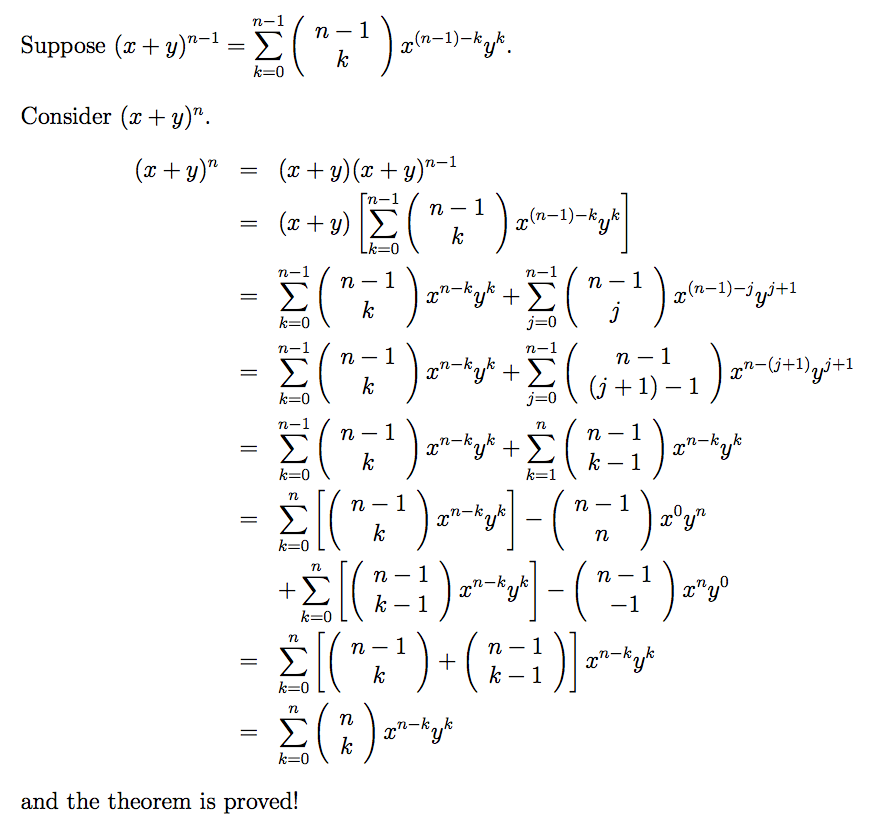
\includegraphics [scale=0.5] {binomial.png}
\end{center}

  It has a number of interesting properties e.g. one can find the Fibonacci numbers from the oblique diagonal.

\end{document}  